%%%%%%%%%%%%%%%%%%%%%%%%%%%%%%%%%%%%%%%%%
% Large Colored Title Article
% LaTeX Template
% Version 1.1 (25/11/12)
%
% This template has been downloaded from:
% http://www.LaTeXTemplates.com
%
% Original author:
% Frits Wenneker (http://www.howtotex.com)
%
% License:
% CC BY-NC-SA 3.0 (http://creativecommons.org/licenses/by-nc-sa/3.0/)
%
%%%%%%%%%%%%%%%%%%%%%%%%%%%%%%%%%%%%%%%%%

%----------------------------------------------------------------------------------------
%	PACKAGES AND OTHER DOCUMENT CONFIGURATIONS
%----------------------------------------------------------------------------------------

\documentclass[DIV=calc, paper=a4, fontsize=11pt]{scrartcl}	 % A4 paper and 11pt font size

\usepackage{lipsum} % Used for inserting dummy 'Lorem ipsum' text into the template
\usepackage[english]{babel} % English language/hyphenation
\usepackage[protrusion=true,expansion=true]{microtype} % Better typography
\usepackage{amsmath,amsfonts,amsthm} % Math packages
\usepackage[svgnames]{xcolor} % Enabling colors by their 'svgnames'
\usepackage[hang, small,labelfont=bf,up,textfont=it,up]{caption} % Custom captions under/above floats in tables or figures
\usepackage{booktabs} % Horizontal rules in tables
\usepackage{fix-cm}	 % Custom font sizes - used for the initial letter in the document

\usepackage{sectsty} % Enables custom subsection titles
%\allsubsectionsfont{\usefont{OT1}{phv}{b}{n}} % Change the font of all subsection commands

\usepackage{fancyhdr} % Needed to define custom headers/footers
\pagestyle{fancy} % Enables the custom headers/footers
\usepackage{lastpage} % Used to determine the number of pages in the document (for "Page X of Total")

\usepackage{fullpage}
\usepackage{graphicx}
\usepackage{pdflscape}
\usepackage{url}

% Headers - all currently empty
\lhead{}
\chead{\footnotesize CS38010 Assignment}
\rhead{}

% Footers
\lfoot{}
\cfoot{\footnotesize adb9}
\rfoot{\footnotesize \thepage\ / \pageref{LastPage}} % "Page 1 of 2"

\renewcommand{\headrulewidth}{0.0pt} % No header rule
\renewcommand{\footrulewidth}{0.4pt} % Thin footer rule

\usepackage{lettrine} % Package to accentuate the first letter of the text
\newcommand{\initial}[1]{ % Defines the command and style for the first letter
\lettrine[lines=3,lhang=0.3,nindent=0em]{
\color{DarkGoldenrod}
{\textsf{#1}}}{}}

%----------------------------------------------------------------------------------------
%	TITLE SECTION
%----------------------------------------------------------------------------------------

\usepackage{titling} % Allows custom title configuration

\newcommand{\HorRule}{\color{DarkGoldenrod} \rule{\linewidth}{1pt}} % Defines the gold horizontal rule around the title

\pretitle{\vspace{-30pt} \begin{flushleft} \HorRule \fontsize{50}{50} \usefont{OT1}{phv}{b}{n} \color{DarkRed} \selectfont} % Horizontal rule before the title

\title{Lorem Ipsum} % Your article title

\posttitle{\par\end{flushleft}\vskip 0.5em} % Whitespace under the title

\preauthor{\begin{flushleft}\large \lineskip 0.5em \usefont{OT1}{phv}{b}{sl} \color{DarkRed}} % Author font configuration

\author{Alexander Brown } % Your name

\postauthor{\footnotesize \usefont{OT1}{phv}{m}{sl} \color{Black} % Configuration for the institution name
(adb9@aber.ac.uk) % Your institution

\par\end{flushleft}\HorRule} % Horizontal rule after the title

\date{} % Add a date here if you would like one to appear underneath the title block

%----------------------------------------------------------------------------------------

\begin{document}

\maketitle % Print the title

\thispagestyle{fancy} % Enabling the custom headers/footers for the first page 

\tableofcontents
\newpage

%----------------------------------------------------------------------------------------
%	ARTICLE CONTENTS
%----------------------------------------------------------------------------------------

\section{Summary}

\subsection{Executive Summary}
Lorem Ispum will sell Customer Relationship Management (CRM) software provided as a service, or
as a privately hosted system. Our CRM software will be fully integrated with all modern mobile
devices from smart-phones to tablets meaning our software can be accessed anywhere with a 
connection to the internet.

Our staff have had intimate knowledge of large scale, distributed systems in their past positions,
as well as good knowledge into managing relationships and CRM software.

\subsection{Business Detail}
\subsubsection*{Company Name}
Lorem Ipsum

\subsubsection*{Address}
42 Lorem Ipsum,\\
Aberystwyth,\\
Ceredigion,\\
England

\subsubsection*{Telephone Number}
+44 1234 987765

\subsubsection*{The Business Will}
The business focuses on agile development of CRM software with a full suite of mobile apps.
% Brief Description


\subsection{Key Personnel}
\subsubsection*{Details of Owners}
\begin{description}
\item[Name:] Alexander Brown
\item[Position and Main Responsibilities:] Director, Software Developer
\item[Experience and Knowledge of our Industry:] 3 years Experience with the Java programming 
language including mobile application and OSGi development. 1 year Linux administration. %TODO
\item[Previous Employment:] CICS L3 Service Tooling Engineer, IBM UK.
\item[Key Skills Brought to the Business:] Software Development and Server Administration.
\item[Academic/Professional Qualifications:] MEng Software Engineering, University of Aberystwyth; 
Java 7 Certification.
\end{description}

\subsubsection*{Other Key Personnel}
\begin{description}
\item[Name:] Mark Richards
\item[Position and Main Responsibilities:] Mobile Developer and Tester
\item[Experience and Knowledge of our Industry:] 5 years Software Development experience in Java, 
C\# and Ruby.
\item[Previous Employment:] Lead Tester, BBC
\item[Key Skills Brought to the Business:] Software Testing and Architecture
\item[Academic/Professions Qualifications:] BSc (Hons) Computer Science, University of Kent
\end{description}

\begin{description}
\item[Name:] Kate Howle
\item[Position and Main Responsibilities:] Systems Administrator and Support
\item[Experience and Knowledge of our Industry:] 7 years UNIX/Linux Administration experience.
\item[Previous Employment:] Senior System Administrator, Linux IT
\item[Key Skills Brought to the Business:] UNIX/Linux Administration
\item[Academic/Professions Qualifications:] BSc (Hons) Computer Science, University of Dublin; 
RedHat Certified Engineer
\end{description}

\begin{description}
\item[Name:] Jay Hans
\item[Position and Main Responsibilities:] Marketing and Sales
\item[Experience and Knowledge of our Industry:] 2 years Marketing
\item[Previous Employment:] Business Analysis, IBM UK
\item[Key Skills Brought to the Business:] Marketing and Sales
\item[Academic/Professions Qualifications:] BSc (Hons) Business Computing, University of Berlin
\end{description}

To start off with we will have to keep salaries low, both mobile and systems developers will be 
paid a slightly lower salary than would be typical. However as the company grows we plan to offer
a rapid increase in wage to increase loyalty.

Our support staff require slightly less skills and their salaries are slightly lower that full
developers. They will also be responsible for the maintenance of our Linux servers on which the 
CRM software is hosted. Again we plan to increase this salary in year 2.

The sales team have a low salary but be working on commission. The marketing manager will be on a
flat salary similar to the developers, again with the aim to rapidly increase this wage.

\section{Vision}

\subsection{Business Ideas}
Lorem Ipsum Inc. will sell Customer Relationship Management (CRM) software services with support
for modern mobile platforms. We offer a good support network to ensure 99.9\% uptime of all of our
systems.

Customers will be able to run our CRM software on their own servers, for which we provide set up
support, or on our own servers, where we guarantee the best possible availability.

Since working in industry we have noticed the poor quality or expense of CRM software which works
whilst on the move. With the availability and prevalence of mobile internet it makes little sense
not to leverage such technologies.

One thing we have also noticed is the lack of choice when it comes to CRM packages. Our aim is to
provide what the customer wants and only charge the customer for what they want.

We will also provide help for any set up of the CRM system and the set up of mobile devices.
% Sum up your business idea

\subsection{Business Goals}
\subsubsection*{First Year of Business}
By the end of the first year we will have a usable system with the basic features implemented and
on sale to customers with support staff. We will also have started the advanced features of our
CRM package, ready to release them by quarter 3 of year 2. 

\subsubsection*{The Business in 5 Years}
In 5 years we will have a full suite of CRM software packages available with hosting on our own
hardware. We will continuously develop our products based on customer feedback in an Agile 
methodology to continue to give customer satisfaction.

\subsection{What the Business Does}
\begin{tabular}{|l|p{0.3\textwidth}|p{0.3\textwidth}|}\hline
Product/Service & Features & Benefits \\ \hline
Contract Monitoring System & Monitoring and Tracking of every stage of the sale process & Streamlines the sale process \\ \hline
Forecasting System & Forecasts into opportunities, territories and sales & Sales forecasts \\ \hline
Social Media Services & Social Media presence to track and communicate with customers & Improves cooperate image \\ \hline
Mobile and Tablet set-up & Set up for mobile devices & On the move access to any of our systems \\ \hline
\end{tabular}


\subsection{What Makes the Business Different}
% Your product/service is unique or different compared with the competition because:
We provide software, support, hosting and set up. We do not restrict the customer and work to 
improve our software to suit their needs.

Our support staff are friendly and knowledgeable and are able to liaise with our developers to get
any problems sorted as quickly as we can.


\subsection{Legal Status}
Lorem Ipsum is a private limited company.

\section{Marketing}

\subsection{Market Research}
% Trends and how you know them
Our market research has shown that cloud-based CRM services will continue to gather popularity.
Cloud is an increasingly popular technology in today's market, especially with the influx of
mobile devices and roaming data.

Our research also shows that customers prefer a clean, customisable interface on which to interact
with CRM software. Again with mobile devices this is especially important with screen real-estate
being a premium.

Social Networking is a great tool to provide our customers to better communicate across the whole
CRM system and with their customers. A large social presence is key to being successful.

These days Google's Android phone operating system is one of the more popular phone operating systems,
iOS from Apple is another very popular phone OS. Emerging OSes like Microsoft Windows Phone and 
Firefox OS are also a market to consider for the not-too-distance future.

\begin{figure}[h]
\centering
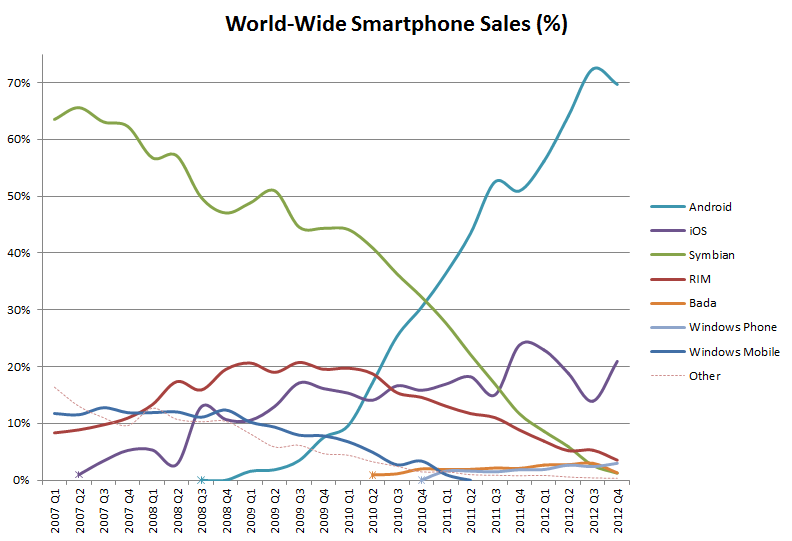
\includegraphics[scale=0.5]{smartphone-sales.png}

From: \url{http://en.wikipedia.org/wiki/File:World_Wide_Smartphone_Sales_Share.png}
\caption{World-Wide Smartphone Sales (\%)} \label{sales}
\end{figure}

Figure~\ref{sales} show the percentage market share of smartphone OSes; from this it is fairly
obvious our main market should be the Android OS, followed by iOS. However, most businesses will
likely have slightly older phones, so RIM (Blackberry) will also be considered. Using an Agile
methodology will also help ease this as we will be able to respond to customers needs rather than
what we believe to be our customers needs.

\subsection{Profiling Customers}
Initially our customers will be small to medium sized businesses that are in the IT industry, 
though we aim to gain popularity and begin to sell our software to larger businesses, while still
catering to smaller ones too.

Working in an Agile fashion we will be able to quickly respond to customer requirements.
% Customer Groups and research

\subsection{Profiling Competitors}
\begin{tabular}{|l|p{0.4\textwidth}|p{0.4\textwidth}|} \hline
Competitor Name & Strengths & Weaknesses \\ \hline
ACT!     & Contract Management    & Entry-level             \\
         & Low cost of investment & Limited number of users \\
         & Easy to use            & Separate Website add-on \\
         & Calendar Management    &  \\
         & Sales Tracking         &  \\
         & Email Merging          &  \\ \hline
GoldMine & Sale force automation  & Complex interface \\
         & Integration Capability & Limited number of users \\
         & Reports and analysis   & Complex set up \\
         & Automated workflows    &  \\
         & Project Management     &  \\
         & Customer service and support &  \\
         & Telemarketing scripting &  \\ \hline
Sage CRM & Ease of use            & Purely website based \\
         & Scalability            & Cost \\
         & Adaptable and Customisable & \\
         & Customer service management & \\
         & Campaign planning and management & \\
         & Performance Reports    & \\ \hline
Microsoft CRM & Automated tools   & Cost \\
         & Embedded with Outlook  & Embedded with Outlook \\ 
         & Reporting Analytics    &  \\
         & Scalability            &  \\
         & Adaptable and Customisable & \\ \hline
\end{tabular}

\subsection{Managing Marketing Risks}
\begin{tabular}{|p{0.5\textwidth}|p{0.5\textwidth}|} \hline
\begin{itemize}
\item Adapting to Customers Feedback
\item Modularity
\item Price
\end{itemize} & 
\begin{itemize}
\item Inexperience
\item Unknown brand
\end{itemize}\\ \hline
\begin{itemize}
\item Emerging Market
\item Mobile Access and Roaming Data
\end{itemize} &
\begin{itemize}
\item Big brands (e.g. Microsoft)
\item Recession
\end{itemize} \\ \hline
\end{tabular}
% I have no idea what I'm doing
% I have no idea what I'm doing
% I have no idea what I'm doing

\section{Pricing}

\begin{tabular}{|l|l|l|} \hline
Product/Service    & Your Price(s) & Range of Competitor Prices (per unit) \\ \hline
CRM Software       & 75 per month (+ extras)  & 280-1134, 26-29 per user per month \\ \hline
Mobile Set Up      & 100           & N/A \\ \hline
Small Business CRM Package & 250   & 280-1134 \\ \hline
Social Media Presence & 40 per month & Included in CRM Software or N/A \\ \hline
Forecasting System & 100 per month & Included in CRM Software or N/A \\ \hline
\end{tabular}

\subsection{Promotion and Advertisement}
% I have no idea what I'm doing
We will mainly focus on marketing our product through networking with potential customers and 
presenting at shows and seminars. Targeted online advertisement will also be used to expand our
clientèle beyond these ranges.

We will also make full use of social media networks to maintain links between new and existing
customers conveniently.

%\subsection{Running the Business}
% I have no idea what I'm doing


\subsection{Staff}
\begin{tabular}{|l|l|l|l|}\hline
Role              & Total Cost & Necessary Experience     & Specialist Skills or Experience \\ \hline
Director          & 20,000     & Java, Project management & Large-scale web-based systems \\ \hline
Systems Developer & 24,000     & Java, C, REST            & Enterprise systems \\ \hline
Mobile Developer  & 24,000     & Java, C\#                & Mobile device application development \\ \hline
Support           & 20,000     & Java, C\#                & Communication \\ \hline
Marketing Manager & 24,000     & Marketing, distribution  & \\ \hline
Sales Team        & 13,000     & Sales                    & \\ \hline
\end{tabular}

\subsection{Premises}
% I have no idea what I'm doing
\begin{tabular}{|l|l|} \hline
                               & Cost (\pounds) \\ \hline
Premises required at start-up: & 6000 (PA)      \\ \hline
\end{tabular}

\subsection{Suppliers}
% I have no idea what I'm doing
\begin{tabular}{|l|l|l|} \hline
Supplier & Product       & Credit \\ \hline
Lenovo   & ThinkPad S430 & 770 \\ \hline
Google   & Nexus 10      & 320 \\ \hline
Apple    & iPad          & 400 \\ \hline
Apple    & Developer License & 67 (PA) \\ \hline
\end{tabular}

\subsection{Equipment}
We will need at least one computer per employee. In today's age it is advantageous to use laptop
computers rather than static desktop machines. This will allow staff to work from any place with
internet access (namely at home or in another office) without inconvenience. We will also invest
in peripheral devices for these machines too.

We will also need to invest in a number of servers on which to host project management software
and, eventually, customer CRM systems. To start with we will rent this from other companies, with
aims to buy our own hardware a few years into the business.

We will try to use Open Source software where possible to minimise the cost. Eclipse, for example,
is a free IDE which is the preferred tool for writing Android applications. Our servers will run
Enterprise Linux (likely RHEL or Cent OS) for which our System Administrator(s) will maintain. 

\subsection{Managing Operational Risks}
Lack of management skill. We will counter this be getting a mentor from our business advisor.

We will have little trading experience, as such it may be difficult to get credit or borrow money,
so we will need to get stakeholders so we can finance the business initially.

Due to a limited number of staff we may come to over-rely on certain members of staff. To begin
with there is no solution to this, but encouraging communication between teams and rotations will
help to ease this in the long run.
% I have no idea what I'm doing

\section{Finance}

\begin{landscape}
\centering
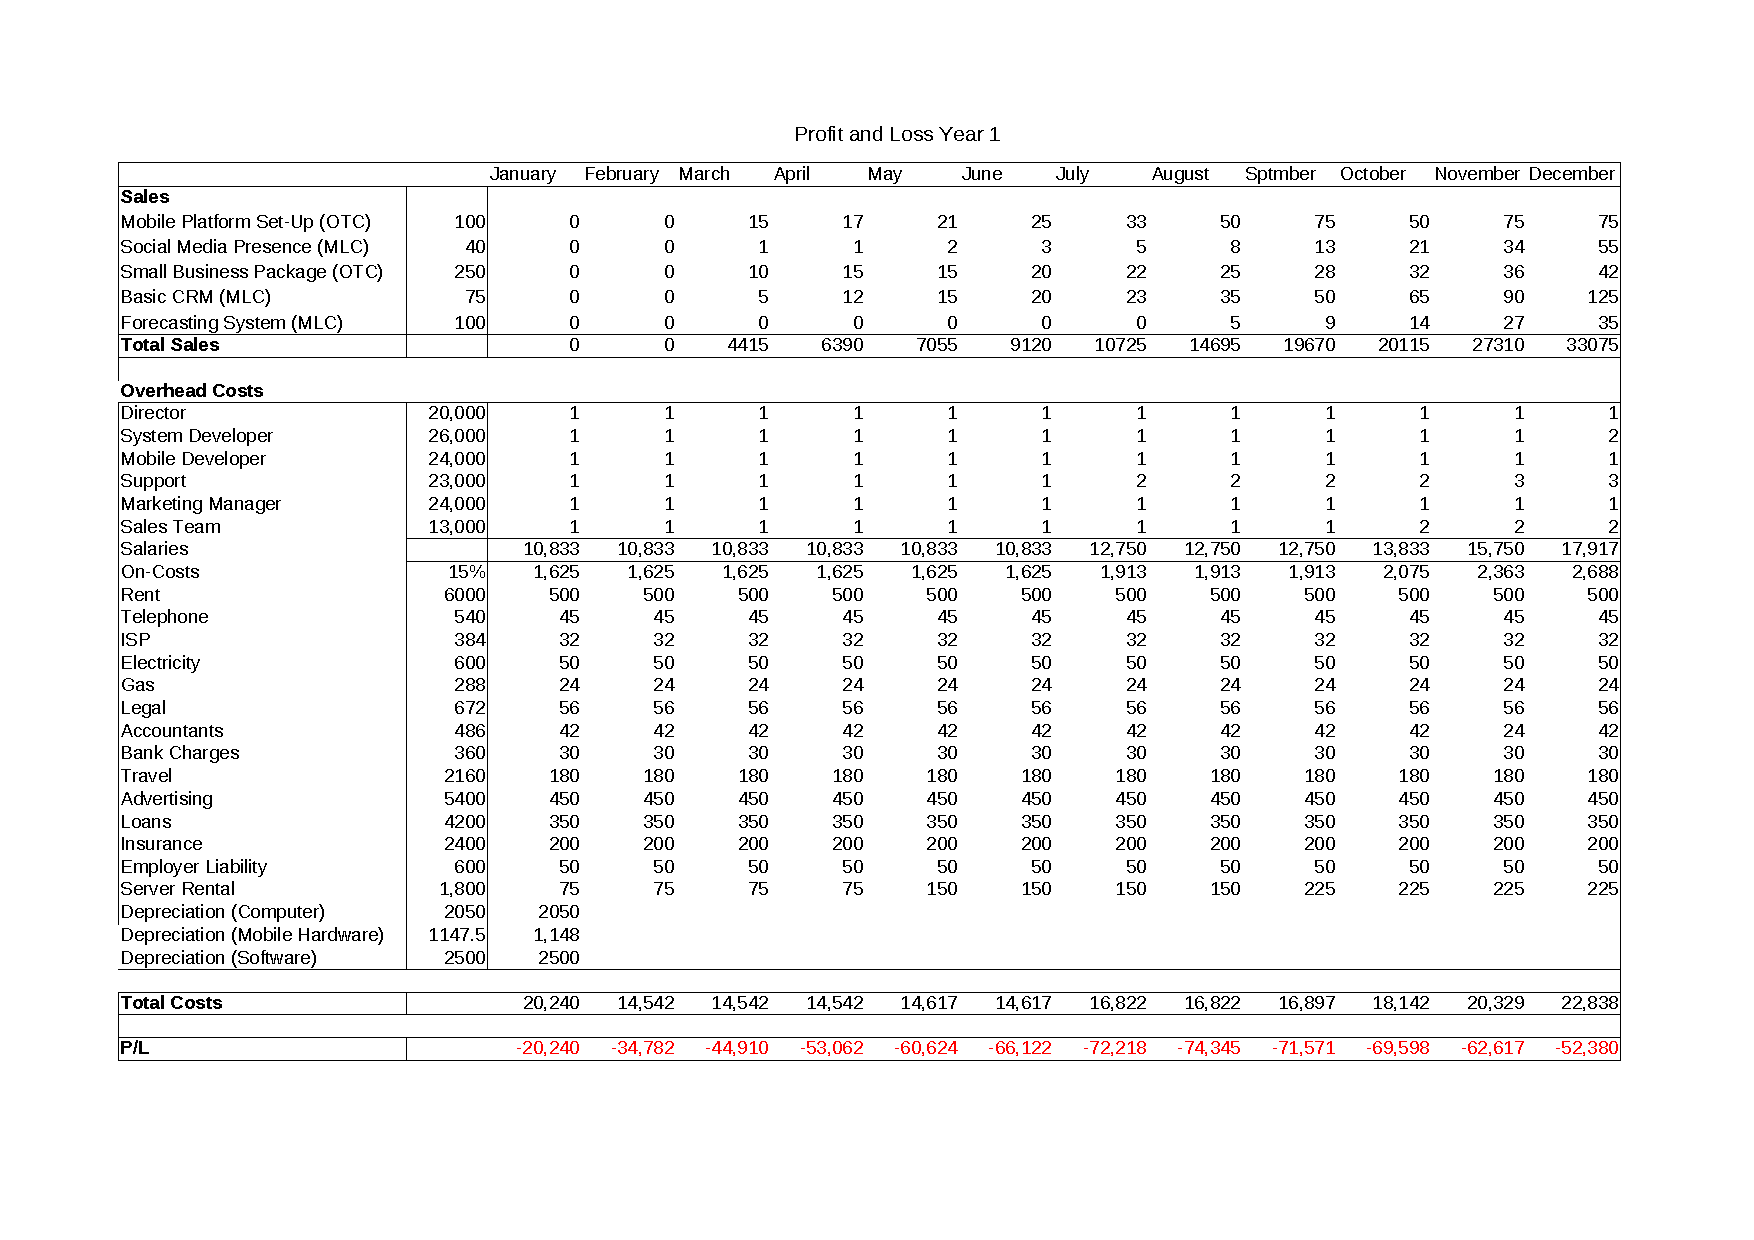
\includegraphics[width=\linewidth]{pl-y1.pdf}
\newpage\hfill\newpage

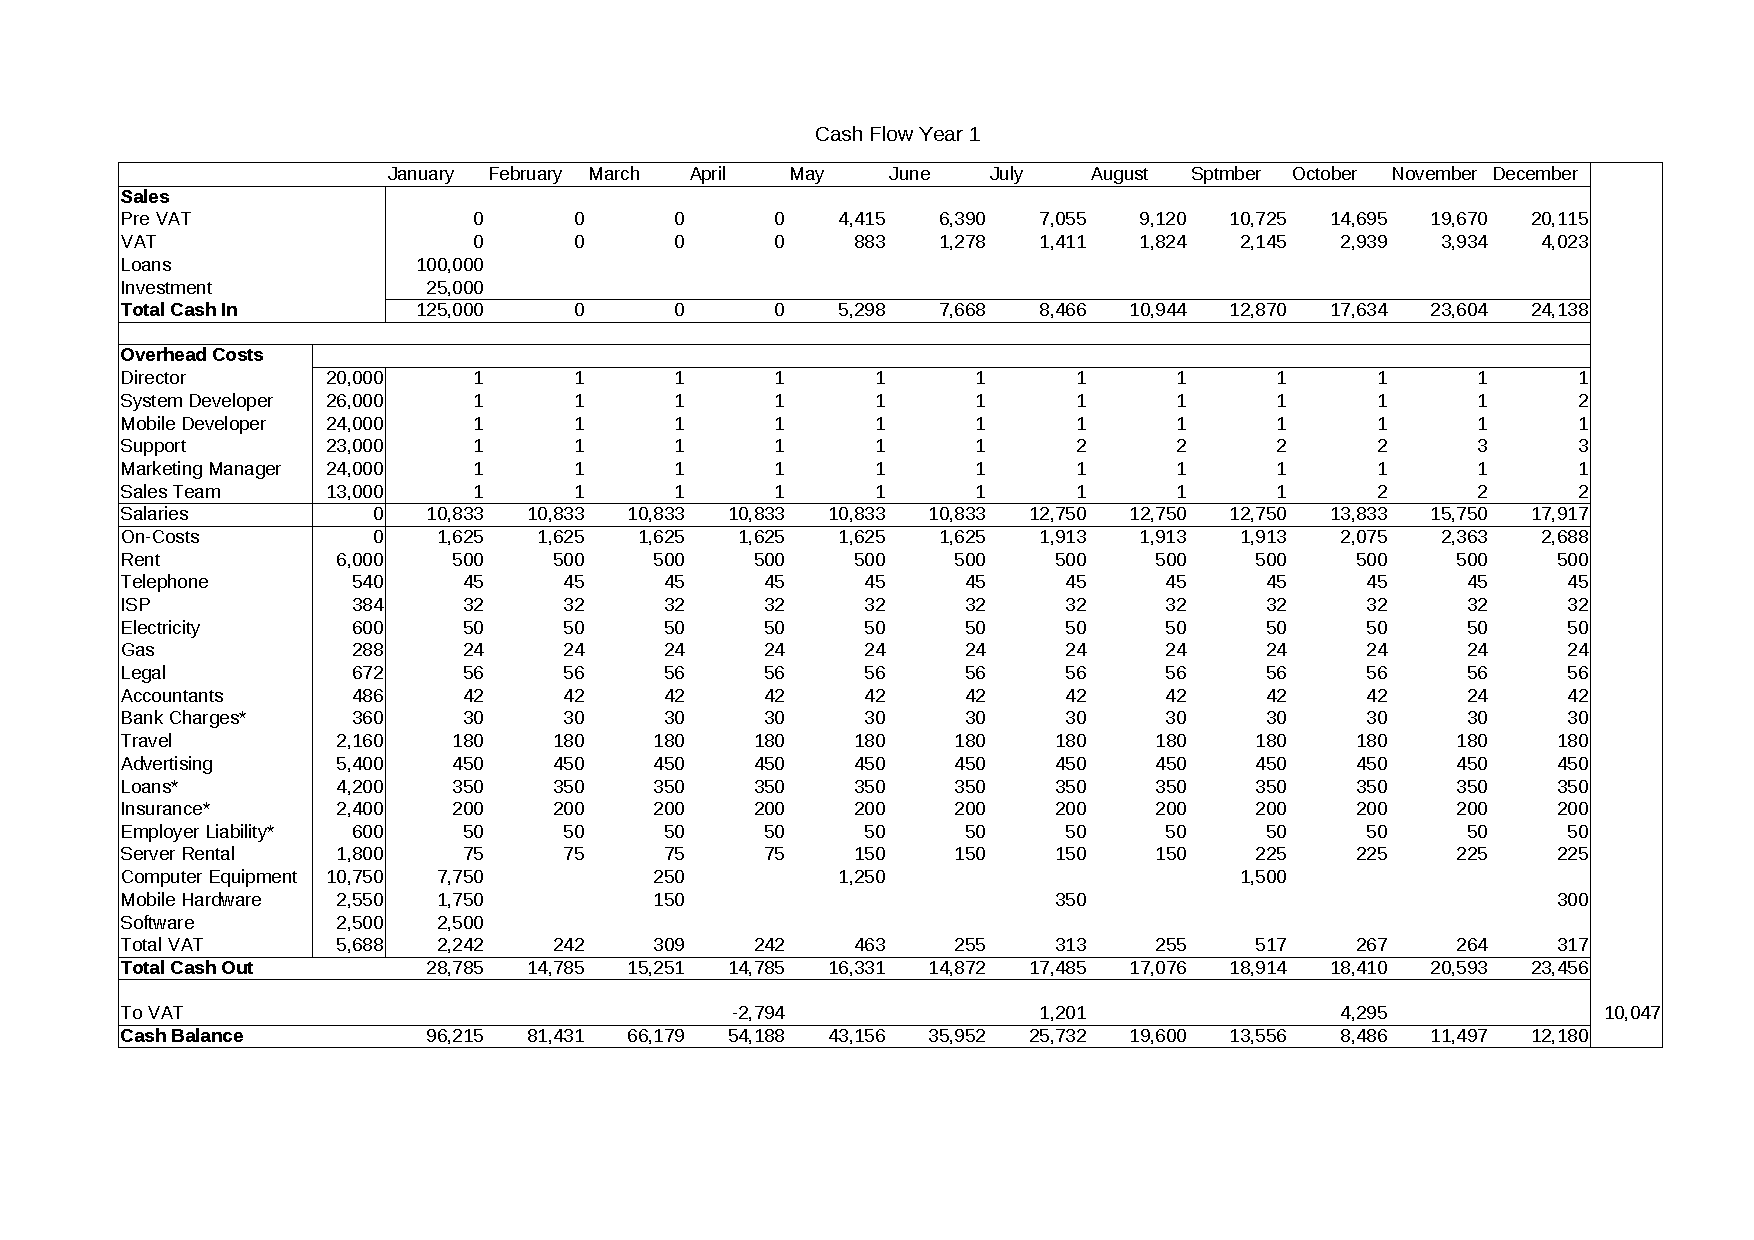
\includegraphics[width=\linewidth]{cashflow-y1.pdf}
\newpage\hfill\newpage

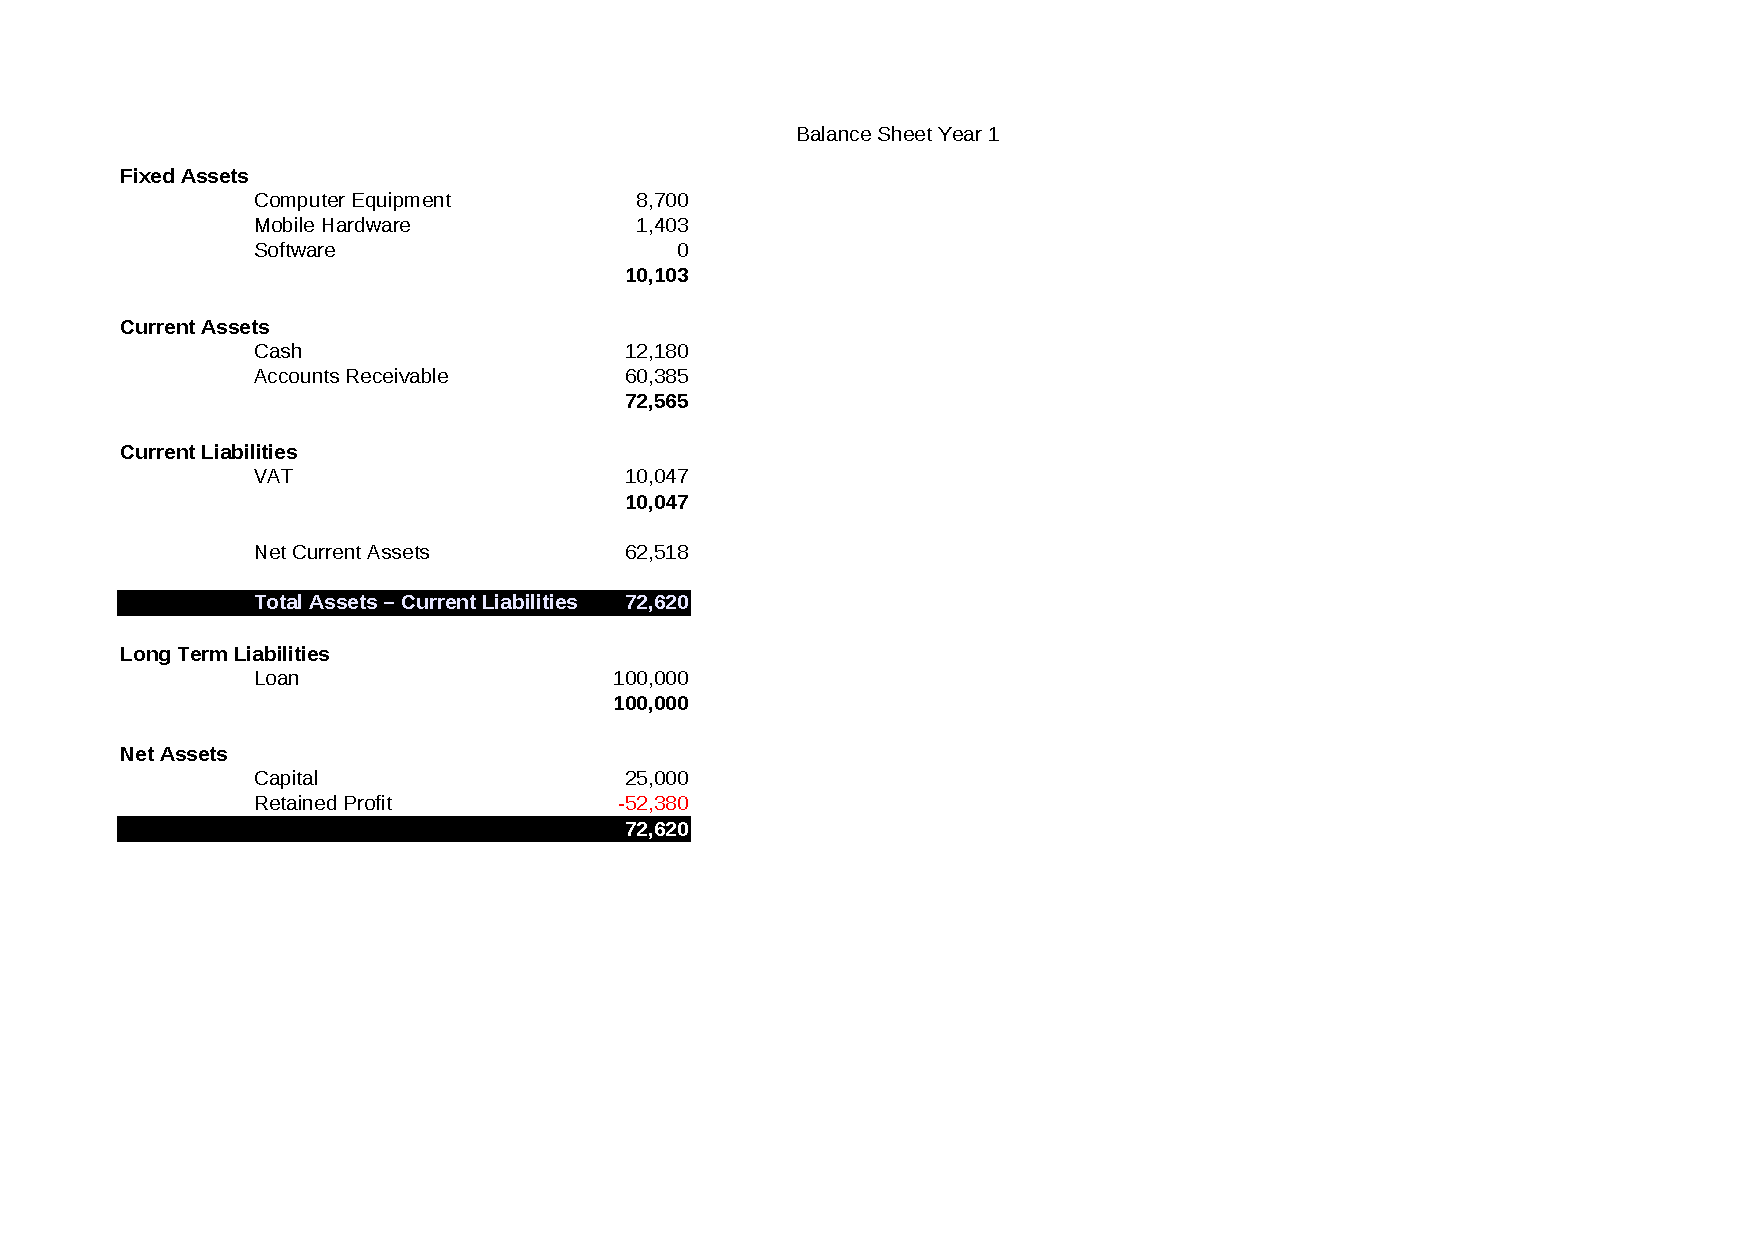
\includegraphics[width=\linewidth]{balance-y1.pdf}
\newpage\hfill\newpage

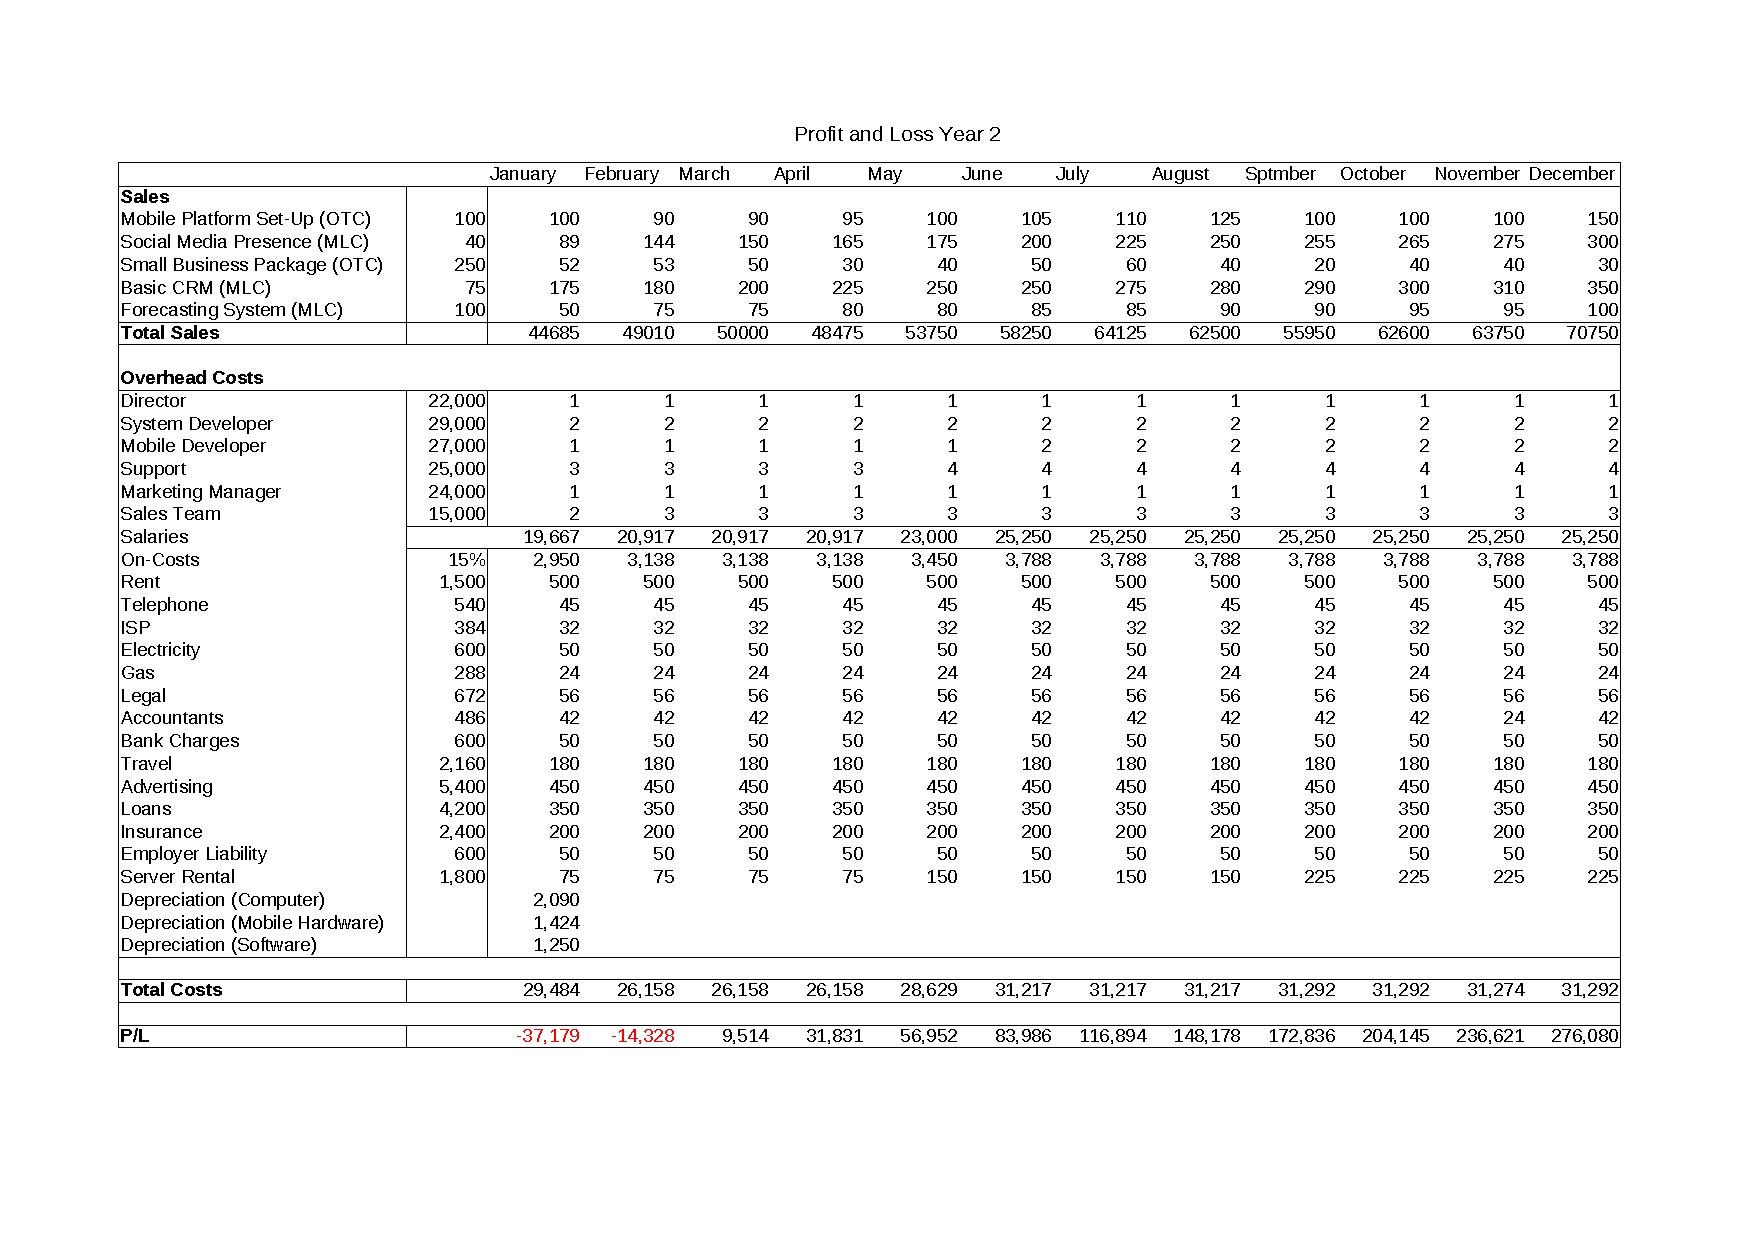
\includegraphics[width=\linewidth]{pl-y2.pdf}
\newpage\hfill\newpage

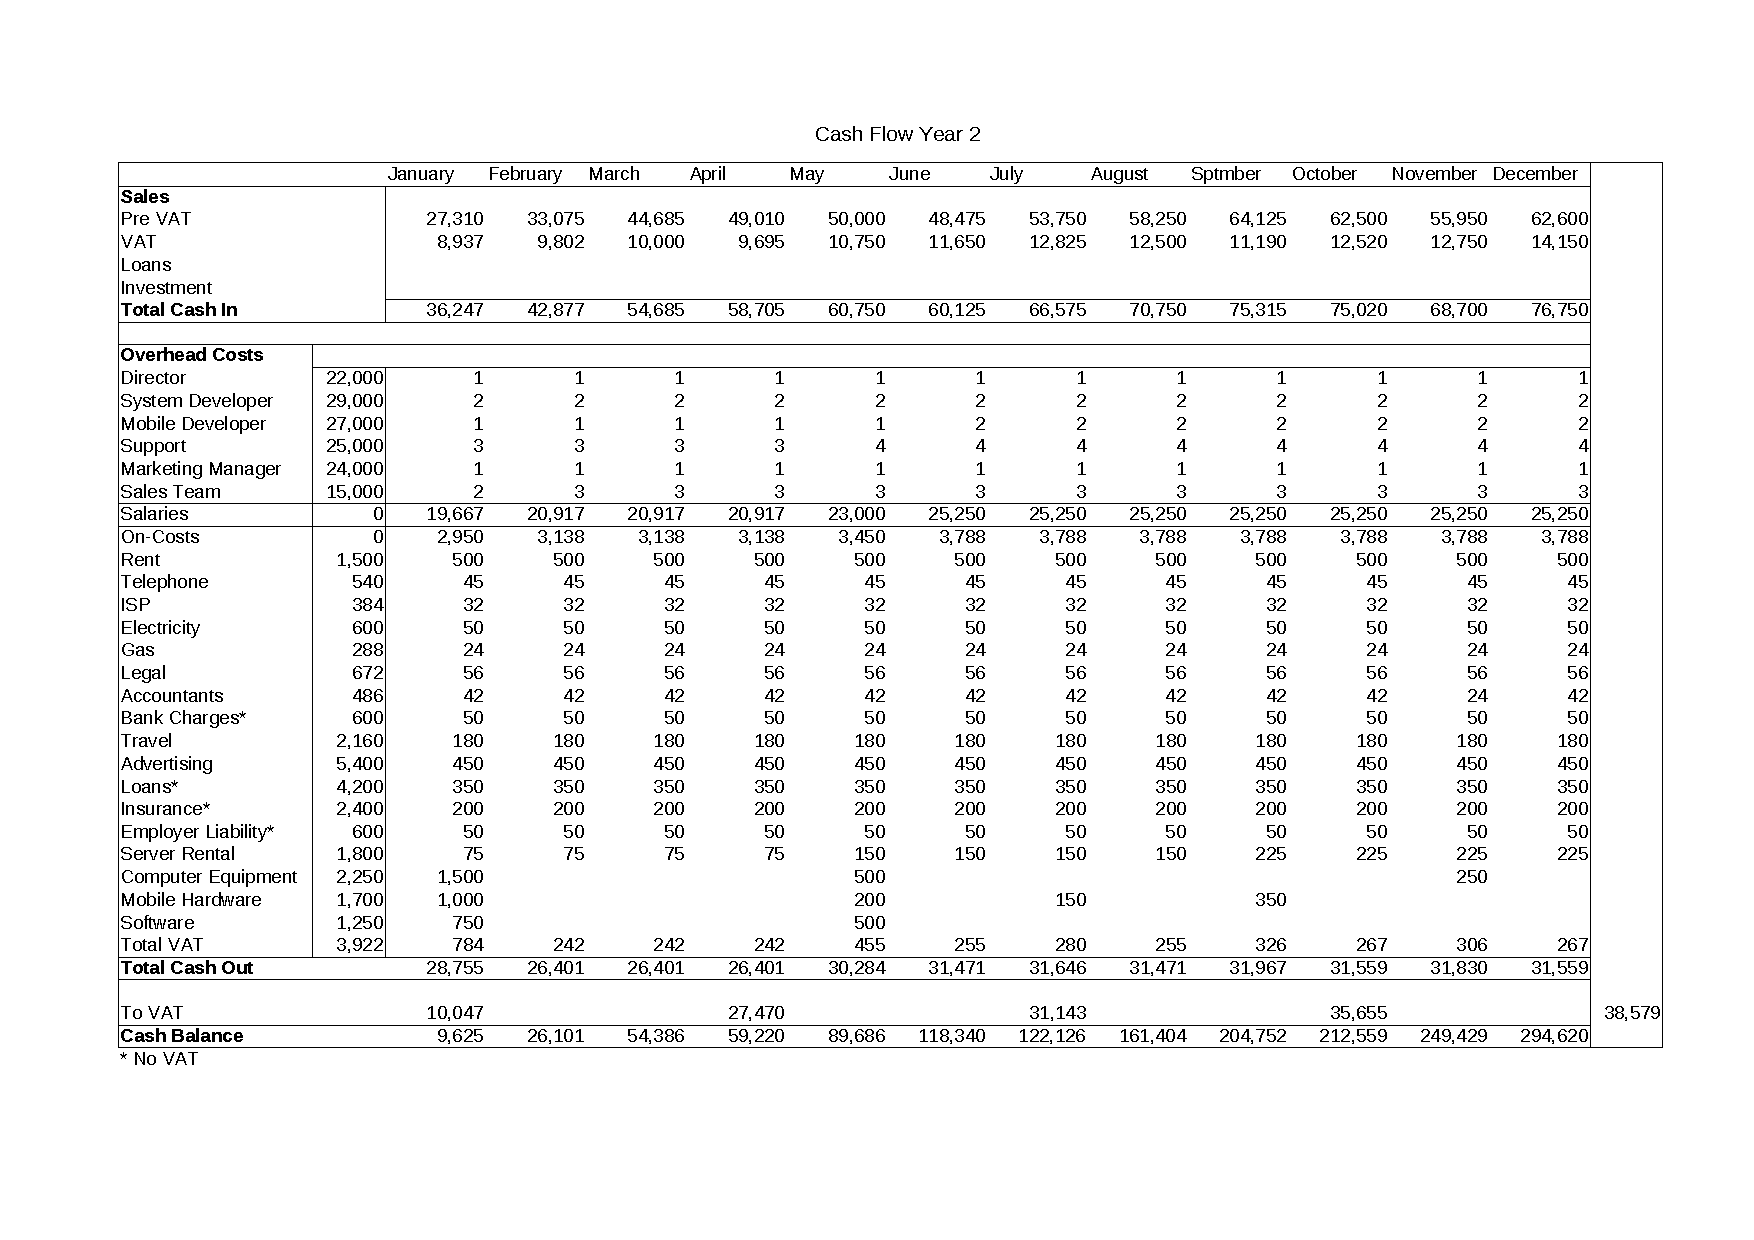
\includegraphics[width=\linewidth]{cashflow-y2.pdf}
\newpage\hfill\newpage

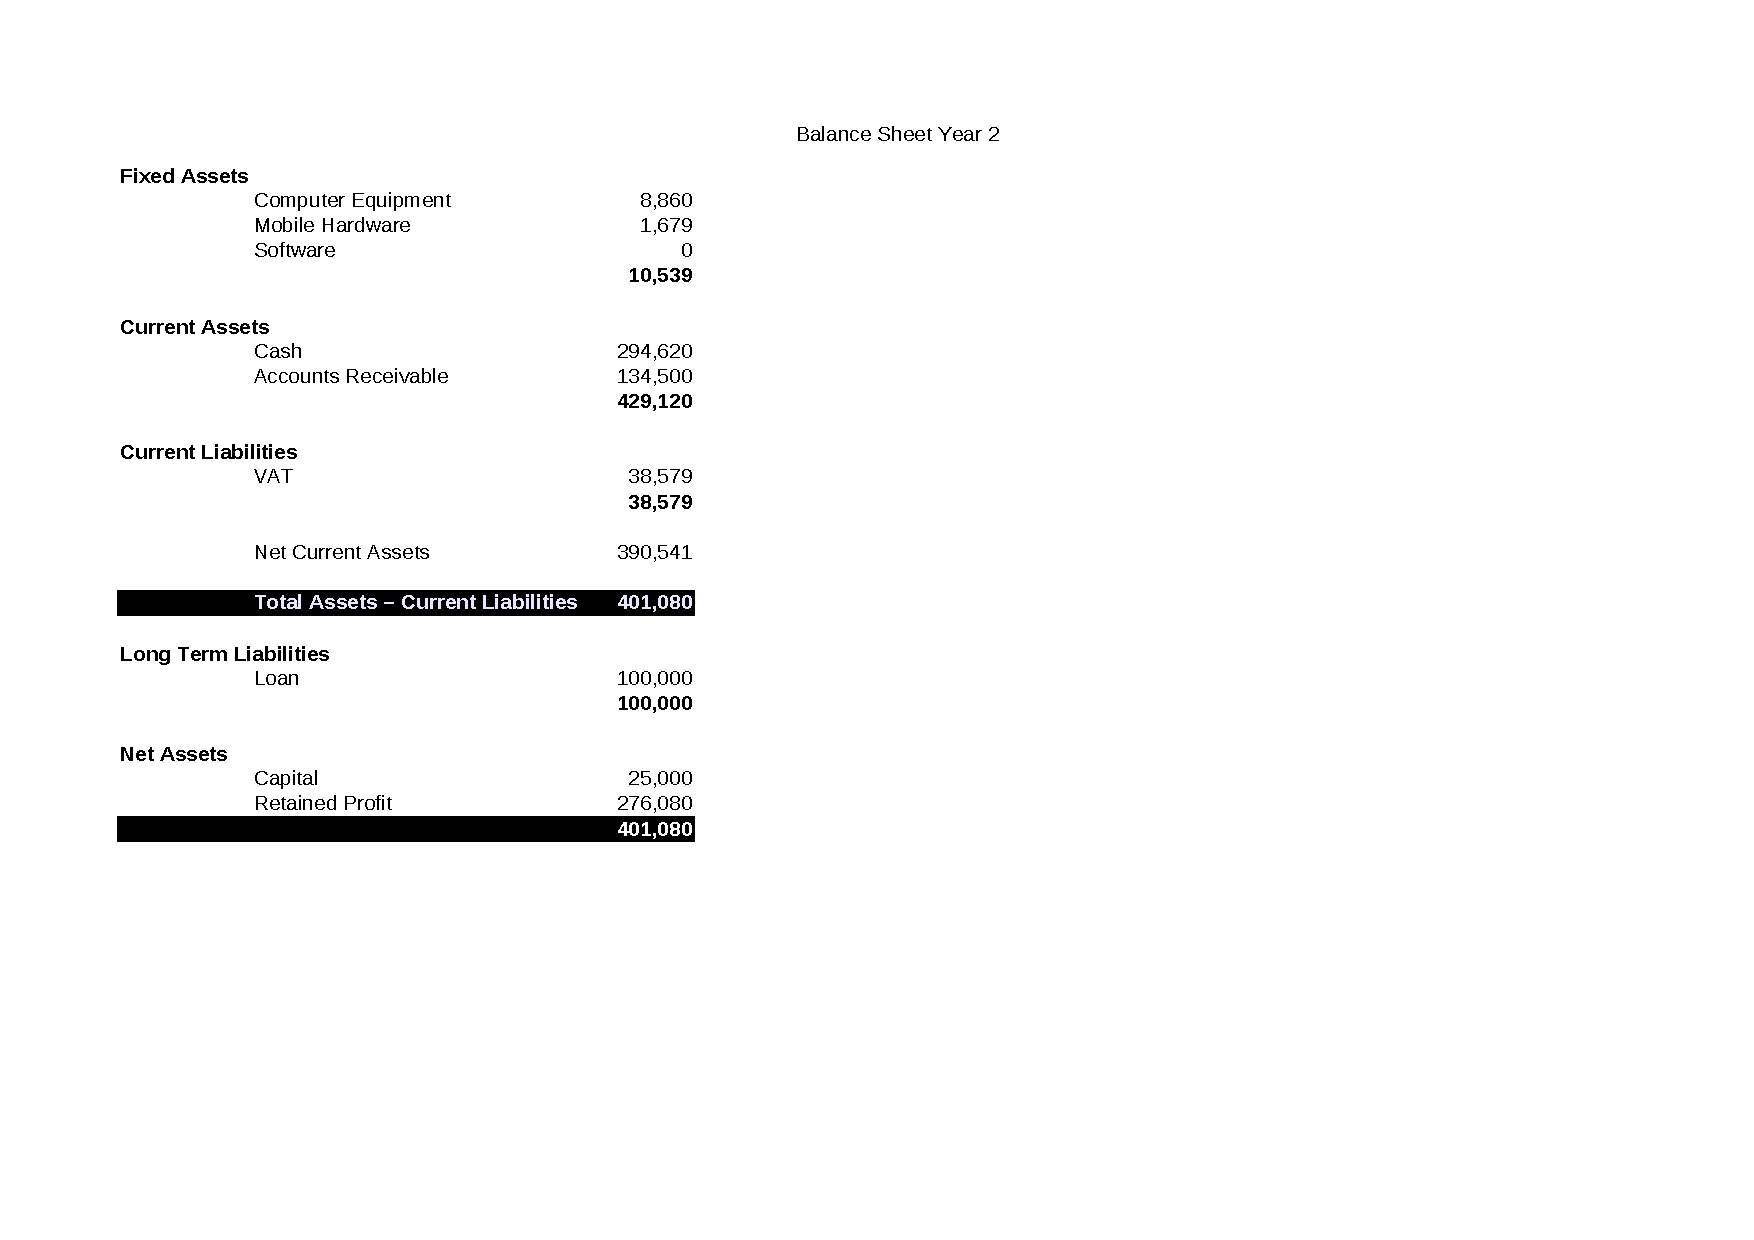
\includegraphics[width=\linewidth]{balance-y2.pdf}
\end{landscape}
\end{document}
